\documentclass{article}
\usepackage{amsmath,amsthm,amsfonts,microtype,amssymb}
\usepackage{enumitem}
\usepackage{parskip}
\usepackage{mathpazo}
\usepackage{tikz-cd}
\usepackage{geometry}
\geometry{top=1in}
\usepackage{float}
\usepackage{graphicx}

\usepackage{hyperref}
\hypersetup{%
  colorlinks=true,
  linkcolor=blue,
  filecolor=blue,
  urlcolor=blue,
  bookmarks=true,
  pdfpagemode=FullScreen,
}


\title{Homework 05 \\ Galois Correspondence of Covering Space}
\author{Algebraic Topology - Winter 2021}
\date{Due: \textbf{March 04, 2021, 11:59 pm}}

\begin{document}
\pagenumbering{gobble}
\maketitle

\begin{enumerate}
\item
  Consider the following commuting diagram between path-connected spaces.
  % the surjectivity of $\ell_1$ is a bit difficult to prove
  % it might be better to just give it as a hypothesis
  \begin{center}
    \begin{tikzcd}
      X \arrow[dr, "\ell_3", swap] \arrow[rr, "\ell_1"]
      && Y \arrow[dl, "\ell_2"]\\
      & Z.
    \end{tikzcd}
  \end{center}
  \begin{enumerate}
  \item Show that if $\ell_2$ and $\ell_3$ are covering maps then so is $\ell_1$.
  \item Find some non-trivial conditions for $\ell_1$ and $\ell_2$ under which if $\ell_1$ and $\ell_2$ are covering
    maps then so is $\ell_3$. Why does \textit{your} proof not work for
    arbitrary $\ell_1$ and $\ell_2$.
  \end{enumerate}
  % \item Construct a 2-fold covering map from a cylinder to a Mobius strip.
  % \item Construct a 2-fold covering map from a torus to a Klein bottle.
\item Classify connected covers, up to isomorphism of covers, of each of the following
  spaces:
  \begin{enumerate}
  \item $\mathbb{RP}^2$,
  \item $\mathbb{RP}^2 \times \mathbb{RP}^2$,
  \item the Mobius strip,
  \item (optional) $\mathbb{RP}^2 \vee \mathbb{RP}^2$.
  \end{enumerate}
  % \begin{figure}[H]
  %   \centering
  %   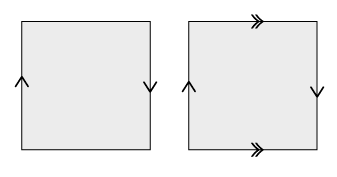
\includegraphics[width=150pt]{images/mobius+klein.png}
  %   \caption{Gluing diagrams of Mobius strip and Klein bottle}
  %   \label{fig:klein_bottle}
  % \end{figure}
\item
  Let $n$ be a positive integer greater than 1. Denote by $\bigvee
  _{n}S^1$ the wedge of $n$ circles at a point.
  \begin{enumerate}
  \item Construct a covering map $\ell: X \to \bigvee _2 S^1$ where $X \simeq \bigvee _n S^1$.
  \item Conclude that there exists an
    inclusion $\mathbb{F}_n \hookrightarrow \mathbb{F}_2$ where $\mathbb{F}_k$ denotes the
    free group on $k$ generators.\footnote{See
      also the \href{https://en.wikipedia.org/wiki/Ping-pong_lemma}{ping-pong lemma}.}
  \item Determine generators and index of $\mathrm{im}(\pi_1(\ell))$ inside
    $\mathbb{F}_2$.
  \item (optional) For what positive integers $m$ does there exist an inclusion
    $\mathbb{F}_m \hookrightarrow \mathbb{F}_n$.
  \item (optional) Show that every subgroup of a free group is free.  \end{enumerate}
\end{enumerate}

\newpage
\section*{Suggested exercises for practice from Hatcher}

\begin{description}
\item[Pg. 79] 1, 2, 4, 8, 10
\item[Pg. 80] 11, 12, 13, 14
\item[Pg. 81] 21, 22
\end{description}

\end{document}
